\section{Introduction}
\label{sec:introduction}

Temporal models can use the past in two ways.  A recurrent model carries an
internal state from one input to the next.  A window model instead receives
recent inputs explicitly and starts each prediction afresh.  These choices
can describe the same input--output behavior, but only if the window contains
the information that still matters to the output.

\begin{figure*}[t]
 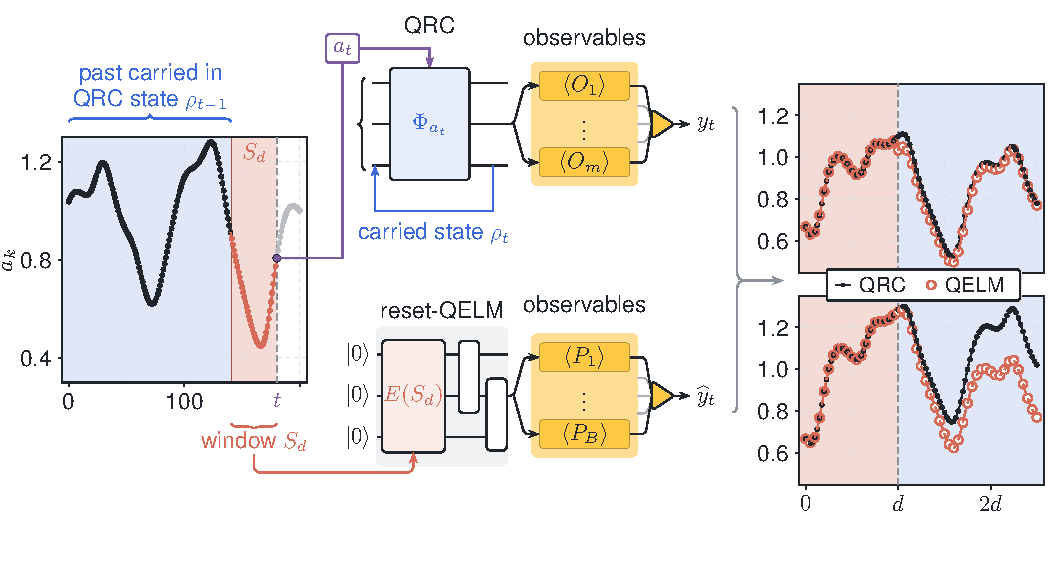
\includegraphics[width=\textwidth]{fig01_information_interface.pdf}
\caption{\textbf{When can finite context replace recurrent quantum memory?}
 \textbf{a} The QRC carries state; the reset-QELM receives the bracketed green window.
 Violet marks current input; grey continuation is excluded.
 Both have model-specific observables and trainable readouts; the target readout stays fixed during emulation.
 Right: the QRC retains an input after it leaves the window. The ideal window predictor
 cannot distinguish its two possible values; green shows their output midpoint for
 one history, not measured QELM performance.
 \textbf{b} For scalar outputs, $D_d/2$ is the smallest worst-case absolute error of
 any window predictor; $D_d$ is the largest output gap between histories sharing
 their last $d$ inputs but differing earlier. Longer windows can reach $\varepsilon$
 unless a higher floor persists. The output example and panel b are schematic.}
 \label{fig:information-interface}
\end{figure*}

Reservoir computing uses fixed internal dynamics and trains only the readout
\cite{maass2002realtime,jaeger2004harnessing,dambre2012information}.  In a
quantum reservoir computer (QRC), a quantum state carries information between
inputs \cite{fujii2017harnessing,mujal2021opportunities}.  A quantum extreme
learning machine (QELM) supplies quantum features to a trainable readout
\cite{huang2006elm,innocenti2023potential}.  Here we consider a reset-window
QELM: it starts from the same state for every prediction and receives only a
finite window of inputs \cite{kawanabe2026tdqelm}.

Imagine two input histories that differ in the distant past but share every
input in that window.  The reset model receives identical data and must make
the same prediction for both.  The QRC can still produce different outputs if
its carried state retains the older difference.  No choice of features,
qubits, training data, or readout can recover information that was not
supplied.  The question is therefore when a finite input window can replace
the part of recurrent memory that affects the desired output.

\par Recurrent quantum reservoirs use persistent dynamics as a temporal
resource in spin networks, noisy processors, oscillators, Rydberg arrays,
Gaussian systems, and quantum-state inputs
\cite{nakajima2019spatial,kutvonen2020optimizing,chen2020temporal,
govia2021oscillator,kalfus2022hilbert,bravo2022rydberg,
nokkala2021gaussian}.  Fading-memory and echo-state results explain when old
state dependence becomes negligible
\cite{boyd1985fading,grigoryeva2018sas,grigoryeva2018esn,
grigoryeva2019differentiable,gonon2021fading,
martinezpena2023finite,martinezpena2025input,kobayashi2024esp,
kobayashi2026coherence}.  Dissipation, feedback, monitored dynamics, and
non-Markovian environments change that memory horizon
\cite{sannia2024dissipation,kobayashi2024feedback,
morguisancho2026monitored,sannia2026nonmarkovian,paparelle2026memory,
ricci2026damping}.

Reset-window models encode recent history explicitly.  Parallel time-delayed
QELMs upload a delay vector, while rewinding and artificial memory restriction
replay a finite suffix from a reset state
\cite{kawanabe2026tdqelm,assil2026memory,mujal2023measurement,
cindrak2024restriction}.  Quantum feature maps can approximate continuous
finite-dimensional functions, including through the repeated-encoding
Bernstein construction used below \cite{goto2021universal,yu2024nonasymptotic}.
Pauli-transfer, Krylov, task-coverage, conditional-information, and Fisher-mode
analyses determine which functions of the supplied window are accessible
\cite{gross2026ptm,cindrak2025krylov,domingo2026diagnosing,keenan2026storage,
wang2026fisher}.  Measurements and finite sampling determine which of those
directions can be resolved
\cite{hu2023sampling,kora2026noise,ahmed2025finite,
mujal2023measurement,morguisancho2026monitored,huang2020shadows}.  We use a
quadratic nonlinear-vector-autoregression model as the strongest classical
delay control \cite{gauthier2021next}.

Decoherence-free subspaces and symmetry-protected steady sectors retain state
components that symmetric dynamics cannot erase
\cite{zanardi1997noiseless,lidar1998dfs,albert2014symmetries}.  Existing results
therefore describe recurrent memory, finite-window representation, and
protected modes separately.  The connection made here is operational: a fixed
window is exact when it contains all information still visible in the declared
QRC output, and growing windows become arbitrarily accurate when the remaining
output gap tends to zero.


We answer this question in two steps.  First, we characterize the smallest
possible error caused by a finite window, independently of the approximating
architecture.  For a scalar output, this error is half the largest output gap
between compatible histories.  Under the continuity, compactness, and
universality assumptions stated in Sec.~\ref{sec:criterion}, a growing
reset-QELM family achieves arbitrary accuracy exactly when that gap vanishes
uniformly as the window grows.  This is an existence result, not a guarantee
that one fixed circuit can learn the map efficiently.

Second, we connect this information limit to the reservoir dynamics.  Only
state differences that past inputs can create and declared outputs can reveal,
now or after later inputs, need to fade.  The internal state need not forget
everything.  We give a dynamical criterion for this relevant forgetting and a
two-qubit example in which symmetry protects an observable memory of an old
input.  The example leaves a nonzero error floor for every finite window.

Held-out simulations then examine what happens with finite windows, features,
and measurements.  These resources address different errors and are not
interchangeable.  A quadratic classical delay model
\cite{gauthier2021next} outperforms the tested fixed QELM on the registered
fast-forgetting comparison, so the experiments do not demonstrate quantum
advantage.  We begin by specifying the two architectures and the output they
are asked to reproduce.
